% UG project example file, February 2024
%
%   Added the "online" option for equal margins, February 2024 [Hiroshi Shimodaira, Iain Murray]
%   A minor change in citation, September 2023 [Hiroshi Shimodaira]
%
% Do not change the first two lines of code, except you may delete "logo," if causing problems.
% Understand any problems and seek approval before assuming it's ok to remove ugcheck.
\documentclass[logo,bsc,singlespacing,parskip,online]{infthesis}
\usepackage{ugcheck}


% Include any packages you need below, but don't include any that change the page
% layout or style of the dissertation. By including the ugcheck package above,
% you should catch most accidental changes of page layout though.

\usepackage{microtype} % recommended, but you can remove if it causes problems

\usepackage{amsmath, amssymb}
\usepackage{xcolor}
\usepackage{tikz}
\usetikzlibrary{shapes.geometric}
\usepackage{graphicx} 

\setlength{\tabcolsep}{4pt}
\newcommand{\pr}[1]{{\scriptsize #1}}          % probability labels
\newcommand{\rd}[1]{\textcolor{red}{$#1$}}      % red cell

\usepackage[numbers]{natbib} % for numerical citations
% \usepackage[round]{natbib} % recommended for citations

\begin{document}
\begin{preliminary}

\title{Database Compression Using Information Theory}

\author{Finlay Peden}

% CHOOSE YOUR DEGREE a):
% please leave just one of the following un-commented
%\course{Artificial Intelligence}
%\course{Artificial Intelligence and Computer Science}
%\course{Artificial Intelligence and Mathematics}
%\course{Artificial Intelligence and Software Engineering}
%\course{Cognitive Science}
%\course{Computer Science}
%\course{Computer Science and Management Science}
%\course{Computer Science and Mathematics}
%\course{Computer Science and Physics}
%\course{Software Engineering}
\course{Master of Informatics} % MInf students

% CHOOSE YOUR DEGREE b):
% please leave just one of the following un-commented
\project{MInf Project (Part 1) Report}  % 4th year MInf students
%\project{MInf Project (Part 2) Report}  % 5th year MInf students
%\project{4th Year Project Report}        % all other UG4 students


\date{\today}

\abstract{
This skeleton demonstrates how to use the \texttt{infthesis} style for
undergraduate dissertations in the School of Informatics. It also emphasises the
page limit, and that you must not deviate from the required style.
The file \texttt{skeleton.tex} generates this document and should be used as a
starting point for your thesis. Replace this abstract text with a concise
summary of your report.
}

\maketitle

\newenvironment{ethics}
   {\begin{frontenv}{Research Ethics Approval}{\LARGE}}
   {\end{frontenv}\newpage}

\begin{ethics}
This project was planned in accordance with the Informatics Research
Ethics policy. It did not involve any aspects that required approval
from the Informatics Research Ethics committee.

\standarddeclaration
\end{ethics}


\begin{acknowledgements}
Any acknowledgements go here.
\end{acknowledgements}


\tableofcontents
\end{preliminary}


\chapter{Introduction}

The preliminary material of your report should contain:
\begin{itemize}
\item
The title page.
\item
An abstract page.
\item
Declaration of ethics and own work.
\item
Optionally an acknowledgements page.
\item
The table of contents.
\end{itemize}

As in this example \texttt{skeleton.tex}, the above material should be
included between:
\begin{verbatim}
\begin{preliminary}
    ...
\end{preliminary}
\end{verbatim}
This style file uses roman numeral page numbers for the preliminary material.

The main content of the dissertation, starting with the first chapter,
starts with page~1. \emph{\textbf{The main content must not go beyond page~40.}}

The report then contains a bibliography and any appendices, which may go beyond
page~40. The appendices are only for any supporting material that's important to
go on record. However, you cannot assume markers of dissertations will read them.

You may not change the dissertation format (e.g., reduce the font size, change
the margins, or reduce the line spacing from the default single spacing). Be
careful if you copy-paste packages into your document preamble from elsewhere.
Some \LaTeX{} packages, such as \texttt{fullpage} or \texttt{savetrees}, change
the margins of your document. Do not include them!

Over-length or incorrectly-formatted dissertations will not be accepted and you
would have to modify your dissertation and resubmit. You cannot assume we will
check your submission before the final deadline and if it requires resubmission
after the deadline to conform to the page and style requirements you will be
subject to the usual late penalties based on your final submission time.

\section{Using Sections}

Divide your chapters into sub-parts as appropriate.

\section{Citations}

When citing work using author names, your sentences should still read
as correct English if any parts in parenthesis are removed.
Use {\tt {\textbackslash}citet} when citing the name as text that's part of your sentence: 
\begin{quote}
  We follow the method of \citet{P1}.
\end{quote}
and use {\tt {\textbackslash}citep} for a parenthetical citation:
\begin{quote}
  It's possible to learn first-order Horn sequences from entailment \citep{P2}.
\end{quote}

You may use any consistent reference style that you prefer, including ``[1]'' numerical citations. 

\chapter{Background}

In this chapter, we will give a general knowledge of the methods needed to understand our proposed compression approach and how to measure its effectiveness. We will start by discussing acyclic schemas along with Multivalued Dependencies (MVDs) and how they will be used to compress the data. We will then explain how the definition of entropy from information theory can be used in determining data loss during the compression. Then we summarize the work by \citet{DBLP:conf/sigmod/KenigMPSS20} in which they describe systems to discover MVDs and Acyclic Join Dependencies. Finally, we will briefly describe widely used database compression techniques. 

To keep consistency we will use the same notation as \citet{DBLP:conf/sigmod/KenigMPSS20}. Let $\Omega$ be a set of variables, also called attributes. If $X , Y \subseteq  \Omega$, then XY denotes $X \cup  Y $.

\section{Running Example}

We will use (Figure~\ref{fig:example}) as an example to demonstrate the information about the background topics. We consider the relation $R$ over the schema $\Omega = \{A,B,C,D\}$. As illustrated, the table $R$ can be decomposed into smaller tables, and joining these tables reconstructs $R$. The join dependency is $R = R[AB] \bowtie R[AC] \bowtie R[BD]$. This dependency only holds for the rows in black. The red rows will be used as an example of approximate acyclic schemas in Section~\ref{MAIMON}.

\begin{figure}[h]
\centering
\noindent\makebox[\textwidth][l]{$R$:}\\[1pt]
\resizebox{\textwidth}{!}{%
\setlength{\tabcolsep}{7pt}%
\begin{tabular}{|c|c|c|c|c}
\cline{1-4}
$A$ & $B$ & $C$ & $D$ & \\ \cline{1-4}
$a_1$ & $b_1$ & $c_1$ & $d_1$ & \pr{1/4} \\
$a_1$ & $b_2$ & $c_1$ & $d_2$ & \pr{1/4} \\
$a_2$ & $b_1$ & $c_2$ & $d_1$ & \pr{1/4} \\
$a_2$ & $b_2$ & $c_2$ & $d_2$ & \pr{1/4} \\
\rd{a_1} & \rd{b_2} & \rd{c_2} & \rd{d_2} &  \\ \cline{1-4}
\end{tabular}
\;$=$\;
\begin{tabular}{|c|c|c}
\cline{1-2}
$A$ & $B$ & \\ \cline{1-2}
$a_1$ & $b_1$ & \pr{1/4} \\
$a_1$ & $b_2$ & \pr{1/4} \\
$a_2$ & $b_1$ & \pr{1/4} \\
$a_2$ & $b_2$ & \pr{1/4} \\ \cline{1-2}
\end{tabular}
\;$\bowtie$\;
\begin{tabular}{|c|c|c}
\cline{1-2}
$A$ & $C$ & \\ \cline{1-2}
$a_1$ & $c_1$ & \pr{1/2} \\
$a_2$ & $c_2$ & \pr{1/2} \\
\rd{a_1} & \rd{c_2} & \\ \cline{1-2}
\end{tabular}
\;$\bowtie$\;
\begin{tabular}{|c|c|c}
\cline{1-2}
$B$ & $D$ & \\ \cline{1-2}
$b_1$ & $d_1$ & \pr{1/2} \\
$b_2$ & $d_2$ & \pr{1/2} \\ \cline{1-2}
\end{tabular}
}
\caption{A relation $R$ and its decomposition into an acyclic schema}
\label{fig:example}
\end{figure}


\section{Acyclic Schemas and Multivalued Dependencies}
In this section, ignore the probabilities (discussed in Sec. \ref{Information Theory}) and the red rows (discussed in Sec. \ref{MAIMON}) in Figure~\ref{fig:example}.

For $Y \subseteq \Omega$ we let $R[Y]$ denote the projection of $R$ onto the attributes $Y$.

When trying to compress databases, it is often useful to decompose a table $R$ with attributes $\Omega$ into smaller tables. A schema is a set $S = \{\Omega_1, \ldots, \Omega_k\}$ of attribute sets whose union is $\Omega$, where no set is contained in another, since a contained set adds no information to the join. $R$ satisfies the join dependency $\mathrm{JD}(S)$, written $R \models \mathrm{JD}(S)$, when joining the projections $R[\Omega_1],\ldots,R[\Omega_k]$ gives us exactly the table $R$. This also means that the decomposition is lossless as joining the projections gives exactly $R$.

An MVD is a special type of join dependency in which, for each value of a set of attributes $X$, the remaining attributes split into groups that vary independently of one another. Let $X,Y_1, \ldots, Y_m \subseteq \Omega$. We say $R$ satisfies the multivalued dependency $X \twoheadrightarrow Y_1 | Y_2 | \ldots | Y_m$  if $R = R[XY_1] \bowtie \cdots \bowtie R[XY_m]$. Where $m\geq 2$, the $Y_i$s are pairwise disjoint and $XY_1 \cdots Y_m = \Omega$. We call $X$ the \emph{key} and $\{Y_1, \ldots, Y_m\}$ the \emph{dependents}. When $m=2$ we call it a \emph{standard MVD} which is the most common form in the literature. 

A schema is \emph{acyclic} if it has a join tree. The schema $\{AB, AC, BD\}$ of Figure~\ref{fig:example} is acyclic, as shown by the join tree in Figure~\ref{fig:jointree}.

\begin{figure}[h]
\centering
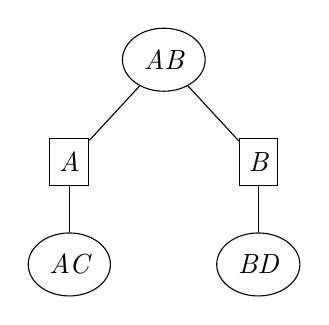
\begin{tikzpicture}[
    every node/.style={font=\itshape},
    rel/.style={draw, ellipse, minimum height=0.8cm},
    sep/.style={draw, rectangle, minimum height=0.6cm},
    level distance=1.3cm]
  \node[rel] (ab) at (0,0)      {AB};
  \node[sep] (a)   at (-1.2,-1.3) {A};
  \node[sep] (b)   at (1.2,-1.3)  {B};
  \node[rel] (ac)  at (-1.2,-2.6) {AC};
  \node[rel] (bd)  at (1.2,-2.6)  {BD};
  \draw (ab) -- (a);
  \draw (ab) -- (b);
  \draw (a)  -- (ac);
  \draw (b)  -- (bd);
\end{tikzpicture}
\caption{Join Tree}
\label{fig:jointree}
\end{figure}

An acyclic schema can be fully described by a set of MVDs, one for each edge of the join tree. The acyclic schema can be described by these two multivalued dependencies: $B \twoheadrightarrow D|AC$, $A \twoheadrightarrow C|BD$. For example the edge $AB \mathrel{\ooalign{$-$\cr\hidewidth$\smash{\raisebox{0.9ex}{$\scriptstyle\mathrm{B}$}}$\hidewidth\cr}} BD$ in the join tree defines the MVD $B \twoheadrightarrow D|AC$. The \emph{separator} of an edge is the intersection of the two bags it joins. Removing an edge splits the tree in two, and the attributes outside the separator split accordingly. The separator and these two groups give an MVD whose key is the separator.

The \emph{separator} of an edge of a join tree is the intersection of the two bags it joins. Removing the edge splits the tree into two subtrees, and the attributes of each subtree that are not in the separator form the two dependents of an MVD whose key is the separator. In Figure~\ref{fig:jointree}, the edge between $AB$ and $BD$ has separator $B$ and gives the MVD $B \twoheadrightarrow D | AC$, and the edge between $AB$ and $AC$ has separator $A$ and gives the MVD $A \twoheadrightarrow C | BD$. Beeri et al.~\cite{DBLP:journals/jacm/BeeriFMY83} showed that $R$ satisfies the acyclic join dependency of the schema exactly when it satisfies the MVD of every edge.

A \emph{join tree} for a schema $S$ is an undirected tree with a set of nodes $\Omega_1, \ldots, \Omega_k $ of S, where the following properties hold: every edge of the graph ($\Omega_i, \Omega_j$) must be labelled with the set of attributes $\Omega_i \cap \Omega_j$ and for all attributes $A$ in $\Omega_i \cap \Omega_j$ each edge along a path between the pair of distinct nodes $\Omega_i, \Omega_j$($\Omega_i \neq \Omega_j$) must include the label $A$ \citep{DBLP:journals/jacm/BeeriFMY83}.

We say that $R$ satisfies the \emph{acyclic join dependency} $\mathrm{AJD}(S)$, written $R \models \mathrm{AJD}(S)$, if the schema $S$ is acyclic and $R \models \mathrm{JD}(S)$. A single MVD $X \twoheadrightarrow Y_1 | \cdots | Y_m$ is the simplest case, since it is the join dependency of the schema $\{XY_1, \ldots, XY_m\}$, whose sets all intersect in $X$. This also explains why one MVD with several dependents is a compact way of writing several standard ones: for example,
$X \twoheadrightarrow A|B|C$ holds exactly when $X \twoheadrightarrow AB|C$, $X \twoheadrightarrow A|BC$ and
$X \twoheadrightarrow AC|B$ all hold \citep{DBLP:conf/sigmod/BeeriFH77}.

The set of MVDs obtained from the edges of a join tree $\mathcal{T}$ is called the \emph{support} of $\mathcal{T}$. Since a tree with $k$ nodes has $k-1$ edges, the support contains $k-1$ MVDs. Because no set of $S$ may be contained in another, an acyclic schema over $n$ attributes has at most $n$ sets \citep{DBLP:journals/jacm/BeeriFMY83}, so a decomposition of $R$ into an acyclic schema never produces more tables than $R$ has attributes. In Figure~\ref{fig:jointree} the support consists of two MVDs and the schema has three sets, which is less than the 4 attributes of $R$.

\section{Information Theory}
\label{Information Theory}

Information theory is the mathematics of quantifying and measuring information. In our context we will be using it to measure the uncertainty in data. Entropy is the main component of information theory that is relevant to this project. It is used to calculate how uncertain a random variable is. 

Let $X$ be a discrete random variable with a set of possible values $\mathcal{X}$ and probability mass function $p(x)$ such that the sum of all probabilities is equal to one. The entropy of X is defined as:
\begin{equation}
  H(X) = \sum_{x \in \mathcal{X}} p(x) \log \frac{1}{p(x)}
  \label{eq:entropy}
\end{equation}

\emph{Mutual Information} is the measure of mutual dependence between two random variables. It equals 0 if an only if the two variables are independent. We write it as:

\begin{equation}
  I(B;C|A) = H(AB) + H(AC) - H(ABC) - H(A)
\end{equation}

Following the work done by \citet{DBLP:journals/tse/Lee87,DBLP:journals/tse/Lee87a} as presented by \citet{DBLP:conf/sigmod/KenigMPSS20}. Let $\mathcal{T}$ be a join tree. We define the following expression:
\begin{equation}
  J(S) = \sum_{i=1}^{n} H(\Omega_i)
       - \sum_{(\Omega_i,\Omega_j)\in \mathrm{edges(\mathcal{T})}} H(\Omega_i \cap \Omega_j)
       - H(\Omega)
  \label{eq:J}
\end{equation}

\section{Mining approximate acyclic schemes from relation}
\label{MAIMON}
MAIMON \citep{DBLP:conf/sigmod/KenigMPSS20}(Multivalued Approximate Inference Mining and NOrmalization) is the system proposed by Kenig et al. to discover MVDs and acyclic schemes in data. They describe enumeration algorithms that allow these discoveries. They also describe a method of calculating the joint entropy of a group of attributes. When evaluating their work they found that this method could be scaled to 1 million rows and 30 attributes with small amounts of spurious tuples. Where a spurious tuple is a row is a tuple not in the original database. Computing the entropy of a set of attributes is the most computationally expensive part of the MAIMON system. Their use of approximate MVDs allowed them to mark more schema as suitable for the compression leading to the compression working even when an exact MVD could not be found. If we now look at the red rows in Figure 2.1 we can see that by adding the row to the original table there now needs to be a new row in the BDE table. However this now means that when the tables are joined together there will be spurious table that was not in the original table. 

If we now look at the red rows in the running example we can see that if we add the 5th red row to R then we also need to add the row $a_1$, $c_1$ in $R[AC]$ as well. However this leads to a spurious tuple in our final result after the joins being a new tuple ($a_1,b_1,c_2,d_1$). In the paper they observe this and note that if only perfect MVDs and acyclic schema were taken then it would not apply widely to databases as if one row in the database changed then the whole schema could no longer be valid. Therefore they chose to use approximate MVDs and acyclic schema instead. 



\section{Database Compression Techniques}
In this section we will give a brief overview of some general database compression techniques that give a better understanding of the topic of database compression and give an option to compress our data further when it can no longer be decomposed using the techniques in \citep{DBLP:conf/sigmod/KenigMPSS20}.

\chapter{Conclusions}

\section{Final Reminder}

The body of your dissertation, before the references and any appendices,
\emph{must} finish by page~40. The introduction, after preliminary material,
should have started on page~1.

You may not change the dissertation format (e.g., reduce the font size, change
the margins, or reduce the line spacing from the default single spacing). Be
careful if you copy-paste packages into your document preamble from elsewhere.
Some \LaTeX{} packages, such as \texttt{fullpage} or \texttt{savetrees}, change
the margins of your document. Do not include them!

Over-length or incorrectly-formatted dissertations will not be accepted and you
would have to modify your dissertation and resubmit. You cannot assume we will
check your submission before the final deadline and if it requires resubmission
after the deadline to conform to the page and style requirements you will be
subject to the usual late penalties based on your final submission time.

% \bibliographystyle{plain}
\bibliographystyle{plainnat}
\bibliography{mybibfile}


% You may delete everything from \appendix up to \end{document} if you don't need it.
\appendix

\chapter{First appendix}

\section{First section}

Any appendices, including any required ethics information, should be included
after the references.

Markers do not have to consider appendices. Make sure that your contributions
are made clear in the main body of the dissertation (within the page limit).

\chapter{Participants' information sheet}

If you had human participants, include key information that they were given in
an appendix, and point to it from the ethics declaration.

\chapter{Participants' consent form}

If you had human participants, include information about how consent was
gathered in an appendix, and point to it from the ethics declaration.
This information is often a copy of a consent form.


\end{document}
